\documentclass[twoside]{book}

% Packages required by doxygen
\usepackage{fixltx2e}
\usepackage{calc}
\usepackage{doxygen}
\usepackage[export]{adjustbox} % also loads graphicx
\usepackage{graphicx}
\usepackage[utf8]{inputenc}
\usepackage{makeidx}
\usepackage{multicol}
\usepackage{multirow}
\PassOptionsToPackage{warn}{textcomp}
\usepackage{textcomp}
\usepackage[nointegrals]{wasysym}
\usepackage[table]{xcolor}

% Font selection
\usepackage[T1]{fontenc}
\usepackage[scaled=.90]{helvet}
\usepackage{courier}
\usepackage{amssymb}
\usepackage{sectsty}
\renewcommand{\familydefault}{\sfdefault}
\allsectionsfont{%
  \fontseries{bc}\selectfont%
  \color{darkgray}%
}
\renewcommand{\DoxyLabelFont}{%
  \fontseries{bc}\selectfont%
  \color{darkgray}%
}
\newcommand{\+}{\discretionary{\mbox{\scriptsize$\hookleftarrow$}}{}{}}

% Page & text layout
\usepackage{geometry}
\geometry{%
  a4paper,%
  top=2.5cm,%
  bottom=2.5cm,%
  left=2.5cm,%
  right=2.5cm%
}
\tolerance=750
\hfuzz=15pt
\hbadness=750
\setlength{\emergencystretch}{15pt}
\setlength{\parindent}{0cm}
\setlength{\parskip}{3ex plus 2ex minus 2ex}
\makeatletter
\renewcommand{\paragraph}{%
  \@startsection{paragraph}{4}{0ex}{-1.0ex}{1.0ex}{%
    \normalfont\normalsize\bfseries\SS@parafont%
  }%
}
\renewcommand{\subparagraph}{%
  \@startsection{subparagraph}{5}{0ex}{-1.0ex}{1.0ex}{%
    \normalfont\normalsize\bfseries\SS@subparafont%
  }%
}
\makeatother

% Headers & footers
\usepackage{fancyhdr}
\pagestyle{fancyplain}
\fancyhead[LE]{\fancyplain{}{\bfseries\thepage}}
\fancyhead[CE]{\fancyplain{}{}}
\fancyhead[RE]{\fancyplain{}{\bfseries\leftmark}}
\fancyhead[LO]{\fancyplain{}{\bfseries\rightmark}}
\fancyhead[CO]{\fancyplain{}{}}
\fancyhead[RO]{\fancyplain{}{\bfseries\thepage}}
\fancyfoot[LE]{\fancyplain{}{}}
\fancyfoot[CE]{\fancyplain{}{}}
\fancyfoot[RE]{\fancyplain{}{\bfseries\scriptsize Generated by Doxygen }}
\fancyfoot[LO]{\fancyplain{}{\bfseries\scriptsize Generated by Doxygen }}
\fancyfoot[CO]{\fancyplain{}{}}
\fancyfoot[RO]{\fancyplain{}{}}
\renewcommand{\footrulewidth}{0.4pt}
\renewcommand{\chaptermark}[1]{%
  \markboth{#1}{}%
}
\renewcommand{\sectionmark}[1]{%
  \markright{\thesection\ #1}%
}

% Indices & bibliography
\usepackage{natbib}
\usepackage[titles]{tocloft}
\setcounter{tocdepth}{3}
\setcounter{secnumdepth}{5}
\makeindex

% Hyperlinks (required, but should be loaded last)
\usepackage{ifpdf}
\ifpdf
  \usepackage[pdftex,pagebackref=true]{hyperref}
\else
  \usepackage[ps2pdf,pagebackref=true]{hyperref}
\fi
\hypersetup{%
  colorlinks=true,%
  linkcolor=blue,%
  citecolor=blue,%
  unicode%
}

% Custom commands
\newcommand{\clearemptydoublepage}{%
  \newpage{\pagestyle{empty}\cleardoublepage}%
}

\usepackage{caption}
\captionsetup{labelsep=space,justification=centering,font={bf},singlelinecheck=off,skip=4pt,position=top}

%===== C O N T E N T S =====

\begin{document}

% Titlepage & ToC
\hypersetup{pageanchor=false,
             bookmarksnumbered=true,
             pdfencoding=unicode
            }
\pagenumbering{alph}
\begin{titlepage}
\vspace*{7cm}
\begin{center}%
{\Large Game of Life }\\
\vspace*{1cm}
{\large Generated by Doxygen 1.8.13}\\
\end{center}
\end{titlepage}
\clearemptydoublepage
\pagenumbering{roman}
\tableofcontents
\clearemptydoublepage
\pagenumbering{arabic}
\hypersetup{pageanchor=true}

%--- Begin generated contents ---
\chapter{File Index}
\section{File List}
Here is a list of all files with brief descriptions\+:\begin{DoxyCompactList}
\item\contentsline{section}{\hyperlink{cunit__t_8c}{cunit\+\_\+t.\+c} }{\pageref{cunit__t_8c}}{}
\item\contentsline{section}{\hyperlink{main_8c}{main.\+c} }{\pageref{main_8c}}{}
\item\contentsline{section}{Drawing/\hyperlink{game_8c}{game.\+c} }{\pageref{game_8c}}{}
\item\contentsline{section}{Drawing/\hyperlink{game_8h}{game.\+h} }{\pageref{game_8h}}{}
\item\contentsline{section}{Drawing/\hyperlink{sdl_8h}{sdl.\+h} }{\pageref{sdl_8h}}{}
\item\contentsline{section}{Game/\hyperlink{arena_8c}{arena.\+c} }{\pageref{arena_8c}}{}
\item\contentsline{section}{Game/\hyperlink{arena_8h}{arena.\+h} }{\pageref{arena_8h}}{}
\item\contentsline{section}{Game/\hyperlink{cell_8c}{cell.\+c} }{\pageref{cell_8c}}{}
\item\contentsline{section}{Game/\hyperlink{cell_8h}{cell.\+h} }{\pageref{cell_8h}}{}
\end{DoxyCompactList}

\chapter{File Documentation}
\hypertarget{cunit__t_8c}{}\section{cunit\+\_\+t.\+c File Reference}
\label{cunit__t_8c}\index{cunit\+\_\+t.\+c@{cunit\+\_\+t.\+c}}
{\ttfamily \#include $<$C\+Unit/\+C\+Unit.\+h$>$}\newline
{\ttfamily \#include $<$C\+Unit/\+Basic.\+h$>$}\newline
{\ttfamily \#include $<$stdio.\+h$>$}\newline
{\ttfamily \#include $<$stdlib.\+h$>$}\newline
{\ttfamily \#include $<$time.\+h$>$}\newline
{\ttfamily \#include \char`\"{}game.\+h\char`\"{}}\newline
{\ttfamily \#include \char`\"{}arena.\+h\char`\"{}}\newline
{\ttfamily \#include \char`\"{}cell.\+h\char`\"{}}\newline
Include dependency graph for cunit\+\_\+t.\+c\+:
\nopagebreak
\begin{figure}[H]
\begin{center}
\leavevmode
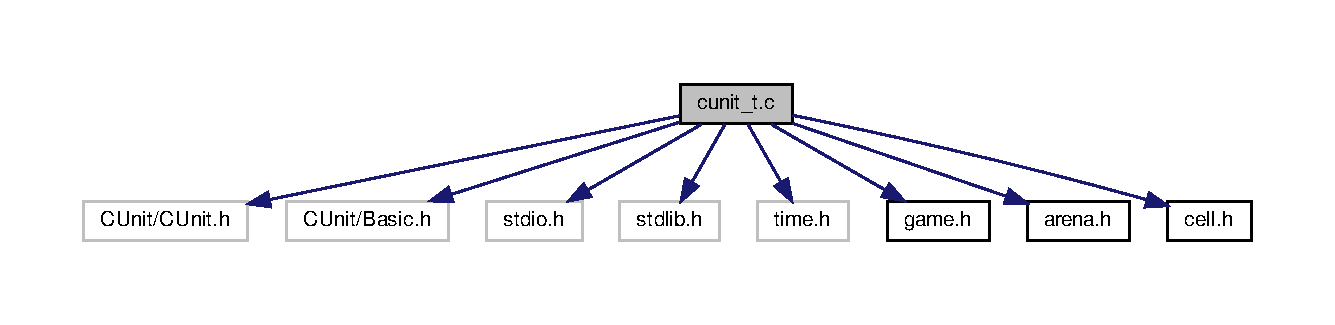
\includegraphics[width=350pt]{cunit__t_8c__incl}
\end{center}
\end{figure}
\subsection*{Functions}
\begin{DoxyCompactItemize}
\item 
void \hyperlink{cunit__t_8c_adb5ff4b2c2410f6ca79e907117e28c0d}{is\+\_\+\+Initialized} (void)
\item 
void \hyperlink{cunit__t_8c_aa56e31fc1daa058dc460b548b39ff4e3}{is\+\_\+\+Generated} (void)
\item 
void \hyperlink{cunit__t_8c_aa5a1771b4b14537b0db0c7a4a813bdc0}{passing\+\_\+by\+\_\+ref\+\_\+check} (void)
\item 
void \hyperlink{cunit__t_8c_a772136466f753a78bba82b04d91173f1}{alive\+\_\+neigh\+\_\+check} (void)
\item 
void \hyperlink{cunit__t_8c_a0f330aafd3a45b823f730ddc4b123728}{cell\+\_\+next\+\_\+step\+\_\+check} (void)
\item 
int \hyperlink{cunit__t_8c_abf9e6b7e6f15df4b525a2e7705ba3089}{main} (int argc, char const $\ast$argv\mbox{[}$\,$\mbox{]})
\end{DoxyCompactItemize}
\subsection*{Variables}
\begin{DoxyCompactItemize}
\item 
int \hyperlink{cunit__t_8c_a439227feff9d7f55384e8780cfc2eb82}{size} =5
\end{DoxyCompactItemize}


\subsection{Function Documentation}
\mbox{\Hypertarget{cunit__t_8c_a772136466f753a78bba82b04d91173f1}\label{cunit__t_8c_a772136466f753a78bba82b04d91173f1}} 
\index{cunit\+\_\+t.\+c@{cunit\+\_\+t.\+c}!alive\+\_\+neigh\+\_\+check@{alive\+\_\+neigh\+\_\+check}}
\index{alive\+\_\+neigh\+\_\+check@{alive\+\_\+neigh\+\_\+check}!cunit\+\_\+t.\+c@{cunit\+\_\+t.\+c}}
\subsubsection{\texorpdfstring{alive\+\_\+neigh\+\_\+check()}{alive\_neigh\_check()}}
{\footnotesize\ttfamily void alive\+\_\+neigh\+\_\+check (\begin{DoxyParamCaption}\item[{void}]{ }\end{DoxyParamCaption})}

\mbox{\Hypertarget{cunit__t_8c_a0f330aafd3a45b823f730ddc4b123728}\label{cunit__t_8c_a0f330aafd3a45b823f730ddc4b123728}} 
\index{cunit\+\_\+t.\+c@{cunit\+\_\+t.\+c}!cell\+\_\+next\+\_\+step\+\_\+check@{cell\+\_\+next\+\_\+step\+\_\+check}}
\index{cell\+\_\+next\+\_\+step\+\_\+check@{cell\+\_\+next\+\_\+step\+\_\+check}!cunit\+\_\+t.\+c@{cunit\+\_\+t.\+c}}
\subsubsection{\texorpdfstring{cell\+\_\+next\+\_\+step\+\_\+check()}{cell\_next\_step\_check()}}
{\footnotesize\ttfamily void cell\+\_\+next\+\_\+step\+\_\+check (\begin{DoxyParamCaption}\item[{void}]{ }\end{DoxyParamCaption})}

\mbox{\Hypertarget{cunit__t_8c_aa56e31fc1daa058dc460b548b39ff4e3}\label{cunit__t_8c_aa56e31fc1daa058dc460b548b39ff4e3}} 
\index{cunit\+\_\+t.\+c@{cunit\+\_\+t.\+c}!is\+\_\+\+Generated@{is\+\_\+\+Generated}}
\index{is\+\_\+\+Generated@{is\+\_\+\+Generated}!cunit\+\_\+t.\+c@{cunit\+\_\+t.\+c}}
\subsubsection{\texorpdfstring{is\+\_\+\+Generated()}{is\_Generated()}}
{\footnotesize\ttfamily void is\+\_\+\+Generated (\begin{DoxyParamCaption}\item[{void}]{ }\end{DoxyParamCaption})}

\mbox{\Hypertarget{cunit__t_8c_adb5ff4b2c2410f6ca79e907117e28c0d}\label{cunit__t_8c_adb5ff4b2c2410f6ca79e907117e28c0d}} 
\index{cunit\+\_\+t.\+c@{cunit\+\_\+t.\+c}!is\+\_\+\+Initialized@{is\+\_\+\+Initialized}}
\index{is\+\_\+\+Initialized@{is\+\_\+\+Initialized}!cunit\+\_\+t.\+c@{cunit\+\_\+t.\+c}}
\subsubsection{\texorpdfstring{is\+\_\+\+Initialized()}{is\_Initialized()}}
{\footnotesize\ttfamily void is\+\_\+\+Initialized (\begin{DoxyParamCaption}\item[{void}]{ }\end{DoxyParamCaption})}

\mbox{\Hypertarget{cunit__t_8c_abf9e6b7e6f15df4b525a2e7705ba3089}\label{cunit__t_8c_abf9e6b7e6f15df4b525a2e7705ba3089}} 
\index{cunit\+\_\+t.\+c@{cunit\+\_\+t.\+c}!main@{main}}
\index{main@{main}!cunit\+\_\+t.\+c@{cunit\+\_\+t.\+c}}
\subsubsection{\texorpdfstring{main()}{main()}}
{\footnotesize\ttfamily int main (\begin{DoxyParamCaption}\item[{int}]{argc,  }\item[{char const $\ast$}]{argv\mbox{[}$\,$\mbox{]} }\end{DoxyParamCaption})}

\mbox{\Hypertarget{cunit__t_8c_aa5a1771b4b14537b0db0c7a4a813bdc0}\label{cunit__t_8c_aa5a1771b4b14537b0db0c7a4a813bdc0}} 
\index{cunit\+\_\+t.\+c@{cunit\+\_\+t.\+c}!passing\+\_\+by\+\_\+ref\+\_\+check@{passing\+\_\+by\+\_\+ref\+\_\+check}}
\index{passing\+\_\+by\+\_\+ref\+\_\+check@{passing\+\_\+by\+\_\+ref\+\_\+check}!cunit\+\_\+t.\+c@{cunit\+\_\+t.\+c}}
\subsubsection{\texorpdfstring{passing\+\_\+by\+\_\+ref\+\_\+check()}{passing\_by\_ref\_check()}}
{\footnotesize\ttfamily void passing\+\_\+by\+\_\+ref\+\_\+check (\begin{DoxyParamCaption}\item[{void}]{ }\end{DoxyParamCaption})}



\subsection{Variable Documentation}
\mbox{\Hypertarget{cunit__t_8c_a439227feff9d7f55384e8780cfc2eb82}\label{cunit__t_8c_a439227feff9d7f55384e8780cfc2eb82}} 
\index{cunit\+\_\+t.\+c@{cunit\+\_\+t.\+c}!size@{size}}
\index{size@{size}!cunit\+\_\+t.\+c@{cunit\+\_\+t.\+c}}
\subsubsection{\texorpdfstring{size}{size}}
{\footnotesize\ttfamily int size =5}


\hypertarget{game_8c}{}\section{Drawing/game.c File Reference}
\label{game_8c}\index{Drawing/game.\+c@{Drawing/game.\+c}}
{\ttfamily \#include $<$stdio.\+h$>$}\newline
{\ttfamily \#include $<$stdlib.\+h$>$}\newline
{\ttfamily \#include $<$time.\+h$>$}\newline
{\ttfamily \#include $<$unistd.\+h$>$}\newline
{\ttfamily \#include \char`\"{}arena.\+h\char`\"{}}\newline
{\ttfamily \#include \char`\"{}cell.\+h\char`\"{}}\newline
{\ttfamily \#include \char`\"{}sdl.\+h\char`\"{}}\newline
{\ttfamily \#include $<$stdint.\+h$>$}\newline
{\ttfamily \#include $<$stdbool.\+h$>$}\newline
{\ttfamily \#include $<$assert.\+h$>$}\newline
Include dependency graph for game.\+c\+:
\nopagebreak
\begin{figure}[H]
\begin{center}
\leavevmode
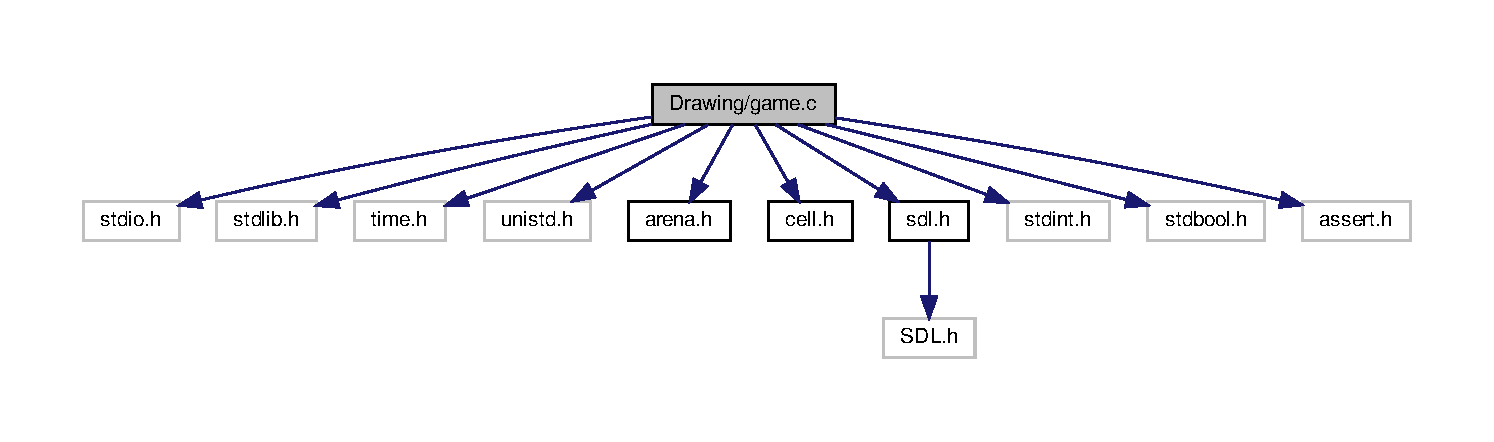
\includegraphics[width=350pt]{game_8c__incl}
\end{center}
\end{figure}
\subsection*{Functions}
\begin{DoxyCompactItemize}
\item 
int $\ast$$\ast$ \hyperlink{game_8c_af9f87e14e073dbe0169f54f2d353c941}{Game\+Step} (int \hyperlink{cunit__t_8c_a439227feff9d7f55384e8780cfc2eb82}{size}, int $\ast$$\ast$game)
\item 
void \hyperlink{game_8c_afa5291b6176515e5611f0230f2794b1b}{play\+Game} (int \hyperlink{cunit__t_8c_a439227feff9d7f55384e8780cfc2eb82}{size}, int $\ast$$\ast$arena)
\item 
void \hyperlink{game_8c_a824a64816df1a405890e7b371a421875}{draw\+\_\+\+S\+DL} (S\+D\+L\+\_\+\+Renderer $\ast$renderer, int $\ast$$\ast$arena, int \hyperlink{cunit__t_8c_a439227feff9d7f55384e8780cfc2eb82}{size})
\item 
void \hyperlink{game_8c_a5931c0456523198ca5c114fba4d0005b}{play\+Game\+\_\+\+S\+DL} (int \hyperlink{cunit__t_8c_a439227feff9d7f55384e8780cfc2eb82}{size}, int $\ast$$\ast$arena)
\end{DoxyCompactItemize}


\subsection{Function Documentation}
\mbox{\Hypertarget{game_8c_a824a64816df1a405890e7b371a421875}\label{game_8c_a824a64816df1a405890e7b371a421875}} 
\index{game.\+c@{game.\+c}!draw\+\_\+\+S\+DL@{draw\+\_\+\+S\+DL}}
\index{draw\+\_\+\+S\+DL@{draw\+\_\+\+S\+DL}!game.\+c@{game.\+c}}
\subsubsection{\texorpdfstring{draw\+\_\+\+S\+D\+L()}{draw\_SDL()}}
{\footnotesize\ttfamily void draw\+\_\+\+S\+DL (\begin{DoxyParamCaption}\item[{S\+D\+L\+\_\+\+Renderer $\ast$}]{renderer,  }\item[{int $\ast$$\ast$}]{arena,  }\item[{int}]{size }\end{DoxyParamCaption})}

\mbox{\Hypertarget{game_8c_af9f87e14e073dbe0169f54f2d353c941}\label{game_8c_af9f87e14e073dbe0169f54f2d353c941}} 
\index{game.\+c@{game.\+c}!Game\+Step@{Game\+Step}}
\index{Game\+Step@{Game\+Step}!game.\+c@{game.\+c}}
\subsubsection{\texorpdfstring{Game\+Step()}{GameStep()}}
{\footnotesize\ttfamily int$\ast$$\ast$ Game\+Step (\begin{DoxyParamCaption}\item[{int}]{size,  }\item[{int $\ast$$\ast$}]{game }\end{DoxyParamCaption})}

\mbox{\Hypertarget{game_8c_afa5291b6176515e5611f0230f2794b1b}\label{game_8c_afa5291b6176515e5611f0230f2794b1b}} 
\index{game.\+c@{game.\+c}!play\+Game@{play\+Game}}
\index{play\+Game@{play\+Game}!game.\+c@{game.\+c}}
\subsubsection{\texorpdfstring{play\+Game()}{playGame()}}
{\footnotesize\ttfamily void play\+Game (\begin{DoxyParamCaption}\item[{int}]{size,  }\item[{int $\ast$$\ast$}]{arena }\end{DoxyParamCaption})}

\mbox{\Hypertarget{game_8c_a5931c0456523198ca5c114fba4d0005b}\label{game_8c_a5931c0456523198ca5c114fba4d0005b}} 
\index{game.\+c@{game.\+c}!play\+Game\+\_\+\+S\+DL@{play\+Game\+\_\+\+S\+DL}}
\index{play\+Game\+\_\+\+S\+DL@{play\+Game\+\_\+\+S\+DL}!game.\+c@{game.\+c}}
\subsubsection{\texorpdfstring{play\+Game\+\_\+\+S\+D\+L()}{playGame\_SDL()}}
{\footnotesize\ttfamily void play\+Game\+\_\+\+S\+DL (\begin{DoxyParamCaption}\item[{int}]{size,  }\item[{int $\ast$$\ast$}]{arena }\end{DoxyParamCaption})}


\hypertarget{game_8h}{}\section{Drawing/game.h File Reference}
\label{game_8h}\index{Drawing/game.\+h@{Drawing/game.\+h}}
This graph shows which files directly or indirectly include this file\+:
\nopagebreak
\begin{figure}[H]
\begin{center}
\leavevmode
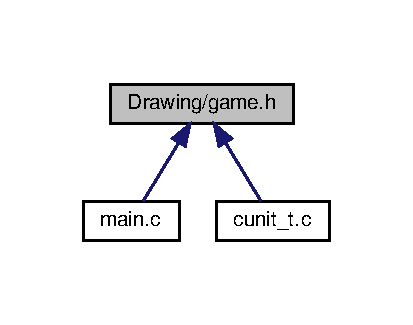
\includegraphics[width=198pt]{game_8h__dep__incl}
\end{center}
\end{figure}
\subsection*{Functions}
\begin{DoxyCompactItemize}
\item 
int $\ast$$\ast$ \hyperlink{game_8h_af9f87e14e073dbe0169f54f2d353c941}{Game\+Step} (int \hyperlink{cunit__t_8c_a439227feff9d7f55384e8780cfc2eb82}{size}, int $\ast$$\ast$game)
\item 
void \hyperlink{game_8h_afa5291b6176515e5611f0230f2794b1b}{play\+Game} (int \hyperlink{cunit__t_8c_a439227feff9d7f55384e8780cfc2eb82}{size}, int $\ast$$\ast$arena)
\end{DoxyCompactItemize}


\subsection{Function Documentation}
\mbox{\Hypertarget{game_8h_af9f87e14e073dbe0169f54f2d353c941}\label{game_8h_af9f87e14e073dbe0169f54f2d353c941}} 
\index{game.\+h@{game.\+h}!Game\+Step@{Game\+Step}}
\index{Game\+Step@{Game\+Step}!game.\+h@{game.\+h}}
\subsubsection{\texorpdfstring{Game\+Step()}{GameStep()}}
{\footnotesize\ttfamily int$\ast$$\ast$ Game\+Step (\begin{DoxyParamCaption}\item[{int}]{size,  }\item[{int $\ast$$\ast$}]{game }\end{DoxyParamCaption})}

\mbox{\Hypertarget{game_8h_afa5291b6176515e5611f0230f2794b1b}\label{game_8h_afa5291b6176515e5611f0230f2794b1b}} 
\index{game.\+h@{game.\+h}!play\+Game@{play\+Game}}
\index{play\+Game@{play\+Game}!game.\+h@{game.\+h}}
\subsubsection{\texorpdfstring{play\+Game()}{playGame()}}
{\footnotesize\ttfamily void play\+Game (\begin{DoxyParamCaption}\item[{int}]{size,  }\item[{int $\ast$$\ast$}]{arena }\end{DoxyParamCaption})}


\hypertarget{sdl_8h}{}\section{Drawing/sdl.h File Reference}
\label{sdl_8h}\index{Drawing/sdl.\+h@{Drawing/sdl.\+h}}
{\ttfamily \#include $<$S\+D\+L.\+h$>$}\newline
Include dependency graph for sdl.\+h\+:
\nopagebreak
\begin{figure}[H]
\begin{center}
\leavevmode
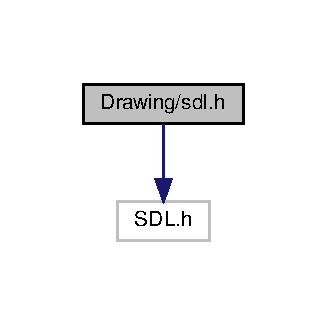
\includegraphics[width=157pt]{sdl_8h__incl}
\end{center}
\end{figure}
This graph shows which files directly or indirectly include this file\+:
\nopagebreak
\begin{figure}[H]
\begin{center}
\leavevmode
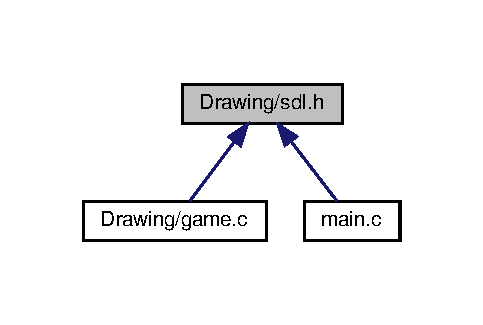
\includegraphics[width=232pt]{sdl_8h__dep__incl}
\end{center}
\end{figure}
\subsection*{Functions}
\begin{DoxyCompactItemize}
\item 
void \hyperlink{sdl_8h_a824a64816df1a405890e7b371a421875}{draw\+\_\+\+S\+DL} (S\+D\+L\+\_\+\+Renderer $\ast$renderer, int $\ast$$\ast$arena, int \hyperlink{cunit__t_8c_a439227feff9d7f55384e8780cfc2eb82}{size})
\item 
void \hyperlink{sdl_8h_a5931c0456523198ca5c114fba4d0005b}{play\+Game\+\_\+\+S\+DL} (int \hyperlink{cunit__t_8c_a439227feff9d7f55384e8780cfc2eb82}{size}, int $\ast$$\ast$arena)
\end{DoxyCompactItemize}


\subsection{Function Documentation}
\mbox{\Hypertarget{sdl_8h_a824a64816df1a405890e7b371a421875}\label{sdl_8h_a824a64816df1a405890e7b371a421875}} 
\index{sdl.\+h@{sdl.\+h}!draw\+\_\+\+S\+DL@{draw\+\_\+\+S\+DL}}
\index{draw\+\_\+\+S\+DL@{draw\+\_\+\+S\+DL}!sdl.\+h@{sdl.\+h}}
\subsubsection{\texorpdfstring{draw\+\_\+\+S\+D\+L()}{draw\_SDL()}}
{\footnotesize\ttfamily void draw\+\_\+\+S\+DL (\begin{DoxyParamCaption}\item[{S\+D\+L\+\_\+\+Renderer $\ast$}]{renderer,  }\item[{int $\ast$$\ast$}]{arena,  }\item[{int}]{size }\end{DoxyParamCaption})}

\mbox{\Hypertarget{sdl_8h_a5931c0456523198ca5c114fba4d0005b}\label{sdl_8h_a5931c0456523198ca5c114fba4d0005b}} 
\index{sdl.\+h@{sdl.\+h}!play\+Game\+\_\+\+S\+DL@{play\+Game\+\_\+\+S\+DL}}
\index{play\+Game\+\_\+\+S\+DL@{play\+Game\+\_\+\+S\+DL}!sdl.\+h@{sdl.\+h}}
\subsubsection{\texorpdfstring{play\+Game\+\_\+\+S\+D\+L()}{playGame\_SDL()}}
{\footnotesize\ttfamily void play\+Game\+\_\+\+S\+DL (\begin{DoxyParamCaption}\item[{int}]{size,  }\item[{int $\ast$$\ast$}]{arena }\end{DoxyParamCaption})}


\hypertarget{arena_8c}{}\section{Game/arena.c File Reference}
\label{arena_8c}\index{Game/arena.\+c@{Game/arena.\+c}}
{\ttfamily \#include $<$stdio.\+h$>$}\newline
{\ttfamily \#include $<$stdlib.\+h$>$}\newline
{\ttfamily \#include $<$time.\+h$>$}\newline
{\ttfamily \#include $<$unistd.\+h$>$}\newline
{\ttfamily \#include \char`\"{}arena.\+h\char`\"{}}\newline
Include dependency graph for arena.\+c\+:
\nopagebreak
\begin{figure}[H]
\begin{center}
\leavevmode
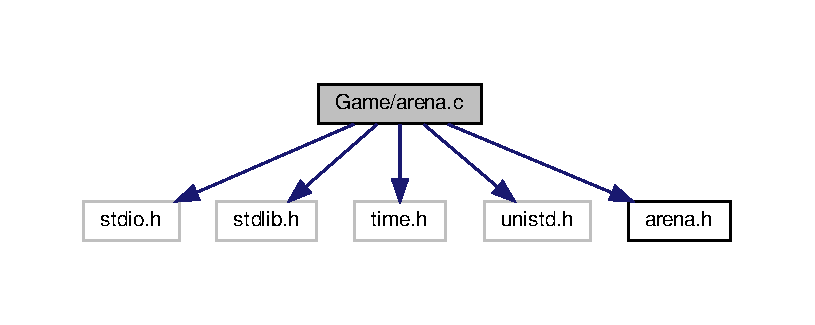
\includegraphics[width=350pt]{arena_8c__incl}
\end{center}
\end{figure}
\subsection*{Functions}
\begin{DoxyCompactItemize}
\item 
int $\ast$$\ast$ \hyperlink{arena_8c_a3c151d7b24b1dcd41fa05c79a4f47c91}{new\+Arena} (int \hyperlink{cunit__t_8c_a439227feff9d7f55384e8780cfc2eb82}{size})
\item 
int $\ast$$\ast$ \hyperlink{arena_8c_a280c814d1796cd5774122d38fb98f7d0}{copy\+Arena} (int \hyperlink{cunit__t_8c_a439227feff9d7f55384e8780cfc2eb82}{size}, int $\ast$$\ast$arena)
\item 
int $\ast$$\ast$ \hyperlink{arena_8c_ae1ccb912a68314effea004a9ea5e2bbc}{random\+Generate} (int \hyperlink{cunit__t_8c_a439227feff9d7f55384e8780cfc2eb82}{size}, int $\ast$$\ast$arena)
\item 
void \hyperlink{arena_8c_a1abde4075f71c301c88a34b20b77e5ce}{print\+Arena\+Digits} (int \hyperlink{cunit__t_8c_a439227feff9d7f55384e8780cfc2eb82}{size}, int $\ast$$\ast$arena)
\end{DoxyCompactItemize}


\subsection{Function Documentation}
\mbox{\Hypertarget{arena_8c_a280c814d1796cd5774122d38fb98f7d0}\label{arena_8c_a280c814d1796cd5774122d38fb98f7d0}} 
\index{arena.\+c@{arena.\+c}!copy\+Arena@{copy\+Arena}}
\index{copy\+Arena@{copy\+Arena}!arena.\+c@{arena.\+c}}
\subsubsection{\texorpdfstring{copy\+Arena()}{copyArena()}}
{\footnotesize\ttfamily int$\ast$$\ast$ copy\+Arena (\begin{DoxyParamCaption}\item[{int}]{size,  }\item[{int $\ast$$\ast$}]{arena }\end{DoxyParamCaption})}

\mbox{\Hypertarget{arena_8c_a3c151d7b24b1dcd41fa05c79a4f47c91}\label{arena_8c_a3c151d7b24b1dcd41fa05c79a4f47c91}} 
\index{arena.\+c@{arena.\+c}!new\+Arena@{new\+Arena}}
\index{new\+Arena@{new\+Arena}!arena.\+c@{arena.\+c}}
\subsubsection{\texorpdfstring{new\+Arena()}{newArena()}}
{\footnotesize\ttfamily int$\ast$$\ast$ new\+Arena (\begin{DoxyParamCaption}\item[{int}]{size }\end{DoxyParamCaption})}

\mbox{\Hypertarget{arena_8c_a1abde4075f71c301c88a34b20b77e5ce}\label{arena_8c_a1abde4075f71c301c88a34b20b77e5ce}} 
\index{arena.\+c@{arena.\+c}!print\+Arena\+Digits@{print\+Arena\+Digits}}
\index{print\+Arena\+Digits@{print\+Arena\+Digits}!arena.\+c@{arena.\+c}}
\subsubsection{\texorpdfstring{print\+Arena\+Digits()}{printArenaDigits()}}
{\footnotesize\ttfamily void print\+Arena\+Digits (\begin{DoxyParamCaption}\item[{int}]{size,  }\item[{int $\ast$$\ast$}]{arena }\end{DoxyParamCaption})}

\mbox{\Hypertarget{arena_8c_ae1ccb912a68314effea004a9ea5e2bbc}\label{arena_8c_ae1ccb912a68314effea004a9ea5e2bbc}} 
\index{arena.\+c@{arena.\+c}!random\+Generate@{random\+Generate}}
\index{random\+Generate@{random\+Generate}!arena.\+c@{arena.\+c}}
\subsubsection{\texorpdfstring{random\+Generate()}{randomGenerate()}}
{\footnotesize\ttfamily int$\ast$$\ast$ random\+Generate (\begin{DoxyParamCaption}\item[{int}]{size,  }\item[{int $\ast$$\ast$}]{arena }\end{DoxyParamCaption})}


\hypertarget{arena_8h}{}\section{Game/arena.h File Reference}
\label{arena_8h}\index{Game/arena.\+h@{Game/arena.\+h}}
This graph shows which files directly or indirectly include this file\+:
\nopagebreak
\begin{figure}[H]
\begin{center}
\leavevmode
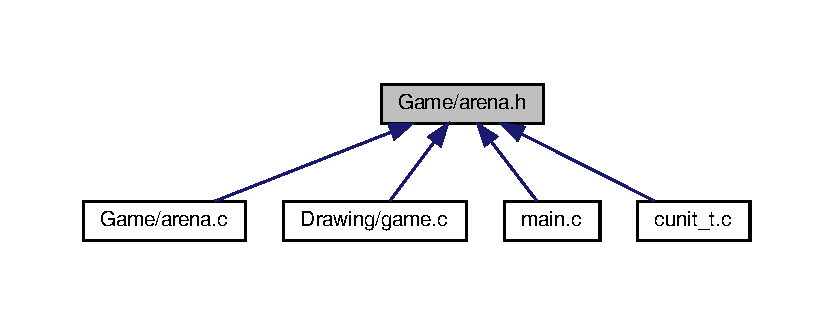
\includegraphics[width=350pt]{arena_8h__dep__incl}
\end{center}
\end{figure}
\subsection*{Functions}
\begin{DoxyCompactItemize}
\item 
int $\ast$$\ast$ \hyperlink{arena_8h_a3c151d7b24b1dcd41fa05c79a4f47c91}{new\+Arena} (int \hyperlink{cunit__t_8c_a439227feff9d7f55384e8780cfc2eb82}{size})
\item 
int $\ast$$\ast$ \hyperlink{arena_8h_a280c814d1796cd5774122d38fb98f7d0}{copy\+Arena} (int \hyperlink{cunit__t_8c_a439227feff9d7f55384e8780cfc2eb82}{size}, int $\ast$$\ast$arena)
\item 
int $\ast$$\ast$ \hyperlink{arena_8h_ae1ccb912a68314effea004a9ea5e2bbc}{random\+Generate} (int \hyperlink{cunit__t_8c_a439227feff9d7f55384e8780cfc2eb82}{size}, int $\ast$$\ast$arena)
\item 
void \hyperlink{arena_8h_a1abde4075f71c301c88a34b20b77e5ce}{print\+Arena\+Digits} (int \hyperlink{cunit__t_8c_a439227feff9d7f55384e8780cfc2eb82}{size}, int $\ast$$\ast$arena)
\end{DoxyCompactItemize}


\subsection{Function Documentation}
\mbox{\Hypertarget{arena_8h_a280c814d1796cd5774122d38fb98f7d0}\label{arena_8h_a280c814d1796cd5774122d38fb98f7d0}} 
\index{arena.\+h@{arena.\+h}!copy\+Arena@{copy\+Arena}}
\index{copy\+Arena@{copy\+Arena}!arena.\+h@{arena.\+h}}
\subsubsection{\texorpdfstring{copy\+Arena()}{copyArena()}}
{\footnotesize\ttfamily int$\ast$$\ast$ copy\+Arena (\begin{DoxyParamCaption}\item[{int}]{size,  }\item[{int $\ast$$\ast$}]{arena }\end{DoxyParamCaption})}

\mbox{\Hypertarget{arena_8h_a3c151d7b24b1dcd41fa05c79a4f47c91}\label{arena_8h_a3c151d7b24b1dcd41fa05c79a4f47c91}} 
\index{arena.\+h@{arena.\+h}!new\+Arena@{new\+Arena}}
\index{new\+Arena@{new\+Arena}!arena.\+h@{arena.\+h}}
\subsubsection{\texorpdfstring{new\+Arena()}{newArena()}}
{\footnotesize\ttfamily int$\ast$$\ast$ new\+Arena (\begin{DoxyParamCaption}\item[{int}]{size }\end{DoxyParamCaption})}

\mbox{\Hypertarget{arena_8h_a1abde4075f71c301c88a34b20b77e5ce}\label{arena_8h_a1abde4075f71c301c88a34b20b77e5ce}} 
\index{arena.\+h@{arena.\+h}!print\+Arena\+Digits@{print\+Arena\+Digits}}
\index{print\+Arena\+Digits@{print\+Arena\+Digits}!arena.\+h@{arena.\+h}}
\subsubsection{\texorpdfstring{print\+Arena\+Digits()}{printArenaDigits()}}
{\footnotesize\ttfamily void print\+Arena\+Digits (\begin{DoxyParamCaption}\item[{int}]{size,  }\item[{int $\ast$$\ast$}]{arena }\end{DoxyParamCaption})}

\mbox{\Hypertarget{arena_8h_ae1ccb912a68314effea004a9ea5e2bbc}\label{arena_8h_ae1ccb912a68314effea004a9ea5e2bbc}} 
\index{arena.\+h@{arena.\+h}!random\+Generate@{random\+Generate}}
\index{random\+Generate@{random\+Generate}!arena.\+h@{arena.\+h}}
\subsubsection{\texorpdfstring{random\+Generate()}{randomGenerate()}}
{\footnotesize\ttfamily int$\ast$$\ast$ random\+Generate (\begin{DoxyParamCaption}\item[{int}]{size,  }\item[{int $\ast$$\ast$}]{arena }\end{DoxyParamCaption})}


\hypertarget{cell_8c}{}\section{Game/cell.c File Reference}
\label{cell_8c}\index{Game/cell.\+c@{Game/cell.\+c}}
{\ttfamily \#include $<$stdio.\+h$>$}\newline
{\ttfamily \#include $<$stdlib.\+h$>$}\newline
{\ttfamily \#include $<$time.\+h$>$}\newline
{\ttfamily \#include $<$unistd.\+h$>$}\newline
{\ttfamily \#include \char`\"{}cell.\+h\char`\"{}}\newline
Include dependency graph for cell.\+c\+:
\nopagebreak
\begin{figure}[H]
\begin{center}
\leavevmode
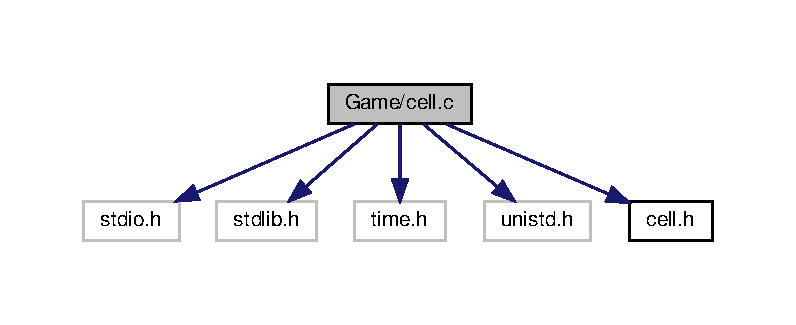
\includegraphics[width=350pt]{cell_8c__incl}
\end{center}
\end{figure}
\subsection*{Functions}
\begin{DoxyCompactItemize}
\item 
int \hyperlink{cell_8c_ac467ed5b4de4c961b67a20a2c142a03f}{sum\+Of\+Neighbors} (int i, int j, int \hyperlink{cunit__t_8c_a439227feff9d7f55384e8780cfc2eb82}{size}, int $\ast$$\ast$arena)
\item 
int \hyperlink{cell_8c_ae67247b9f15b1afd534edd7d39f85bf0}{cell\+Situation} (int i, int j, int \hyperlink{cunit__t_8c_a439227feff9d7f55384e8780cfc2eb82}{size}, int $\ast$$\ast$arena)
\end{DoxyCompactItemize}


\subsection{Function Documentation}
\mbox{\Hypertarget{cell_8c_ae67247b9f15b1afd534edd7d39f85bf0}\label{cell_8c_ae67247b9f15b1afd534edd7d39f85bf0}} 
\index{cell.\+c@{cell.\+c}!cell\+Situation@{cell\+Situation}}
\index{cell\+Situation@{cell\+Situation}!cell.\+c@{cell.\+c}}
\subsubsection{\texorpdfstring{cell\+Situation()}{cellSituation()}}
{\footnotesize\ttfamily int cell\+Situation (\begin{DoxyParamCaption}\item[{int}]{i,  }\item[{int}]{j,  }\item[{int}]{size,  }\item[{int $\ast$$\ast$}]{arena }\end{DoxyParamCaption})}

\mbox{\Hypertarget{cell_8c_ac467ed5b4de4c961b67a20a2c142a03f}\label{cell_8c_ac467ed5b4de4c961b67a20a2c142a03f}} 
\index{cell.\+c@{cell.\+c}!sum\+Of\+Neighbors@{sum\+Of\+Neighbors}}
\index{sum\+Of\+Neighbors@{sum\+Of\+Neighbors}!cell.\+c@{cell.\+c}}
\subsubsection{\texorpdfstring{sum\+Of\+Neighbors()}{sumOfNeighbors()}}
{\footnotesize\ttfamily int sum\+Of\+Neighbors (\begin{DoxyParamCaption}\item[{int}]{i,  }\item[{int}]{j,  }\item[{int}]{size,  }\item[{int $\ast$$\ast$}]{arena }\end{DoxyParamCaption})}


\hypertarget{cell_8h}{}\section{Game/cell.h File Reference}
\label{cell_8h}\index{Game/cell.\+h@{Game/cell.\+h}}
This graph shows which files directly or indirectly include this file\+:
\nopagebreak
\begin{figure}[H]
\begin{center}
\leavevmode
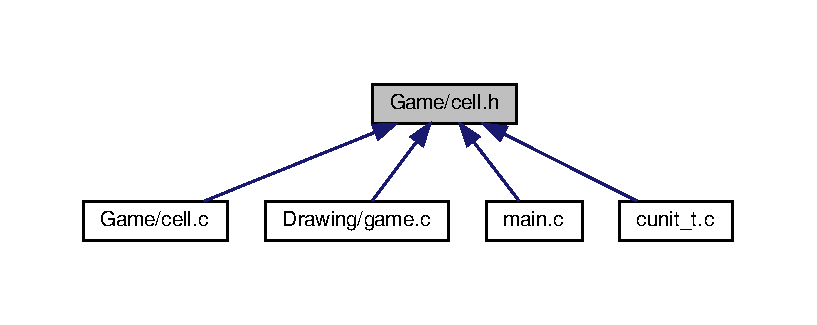
\includegraphics[width=350pt]{cell_8h__dep__incl}
\end{center}
\end{figure}
\subsection*{Functions}
\begin{DoxyCompactItemize}
\item 
int \hyperlink{cell_8h_ac467ed5b4de4c961b67a20a2c142a03f}{sum\+Of\+Neighbors} (int i, int j, int \hyperlink{cunit__t_8c_a439227feff9d7f55384e8780cfc2eb82}{size}, int $\ast$$\ast$arena)
\item 
int \hyperlink{cell_8h_ae67247b9f15b1afd534edd7d39f85bf0}{cell\+Situation} (int i, int j, int \hyperlink{cunit__t_8c_a439227feff9d7f55384e8780cfc2eb82}{size}, int $\ast$$\ast$arena)
\end{DoxyCompactItemize}
\subsection*{Variables}
\begin{DoxyCompactItemize}
\item 
int \hyperlink{cell_8h_ac765329451135abec74c45e1897abf26}{type}
\end{DoxyCompactItemize}


\subsection{Function Documentation}
\mbox{\Hypertarget{cell_8h_ae67247b9f15b1afd534edd7d39f85bf0}\label{cell_8h_ae67247b9f15b1afd534edd7d39f85bf0}} 
\index{cell.\+h@{cell.\+h}!cell\+Situation@{cell\+Situation}}
\index{cell\+Situation@{cell\+Situation}!cell.\+h@{cell.\+h}}
\subsubsection{\texorpdfstring{cell\+Situation()}{cellSituation()}}
{\footnotesize\ttfamily int cell\+Situation (\begin{DoxyParamCaption}\item[{int}]{i,  }\item[{int}]{j,  }\item[{int}]{size,  }\item[{int $\ast$$\ast$}]{arena }\end{DoxyParamCaption})}

\mbox{\Hypertarget{cell_8h_ac467ed5b4de4c961b67a20a2c142a03f}\label{cell_8h_ac467ed5b4de4c961b67a20a2c142a03f}} 
\index{cell.\+h@{cell.\+h}!sum\+Of\+Neighbors@{sum\+Of\+Neighbors}}
\index{sum\+Of\+Neighbors@{sum\+Of\+Neighbors}!cell.\+h@{cell.\+h}}
\subsubsection{\texorpdfstring{sum\+Of\+Neighbors()}{sumOfNeighbors()}}
{\footnotesize\ttfamily int sum\+Of\+Neighbors (\begin{DoxyParamCaption}\item[{int}]{i,  }\item[{int}]{j,  }\item[{int}]{size,  }\item[{int $\ast$$\ast$}]{arena }\end{DoxyParamCaption})}



\subsection{Variable Documentation}
\mbox{\Hypertarget{cell_8h_ac765329451135abec74c45e1897abf26}\label{cell_8h_ac765329451135abec74c45e1897abf26}} 
\index{cell.\+h@{cell.\+h}!type@{type}}
\index{type@{type}!cell.\+h@{cell.\+h}}
\subsubsection{\texorpdfstring{type}{type}}
{\footnotesize\ttfamily int type}


\hypertarget{main_8c}{}\section{main.\+c File Reference}
\label{main_8c}\index{main.\+c@{main.\+c}}
{\ttfamily \#include $<$stdio.\+h$>$}\newline
{\ttfamily \#include $<$stdlib.\+h$>$}\newline
{\ttfamily \#include \char`\"{}game.\+h\char`\"{}}\newline
{\ttfamily \#include \char`\"{}arena.\+h\char`\"{}}\newline
{\ttfamily \#include \char`\"{}cell.\+h\char`\"{}}\newline
{\ttfamily \#include \char`\"{}sdl.\+h\char`\"{}}\newline
Include dependency graph for main.\+c\+:
\nopagebreak
\begin{figure}[H]
\begin{center}
\leavevmode
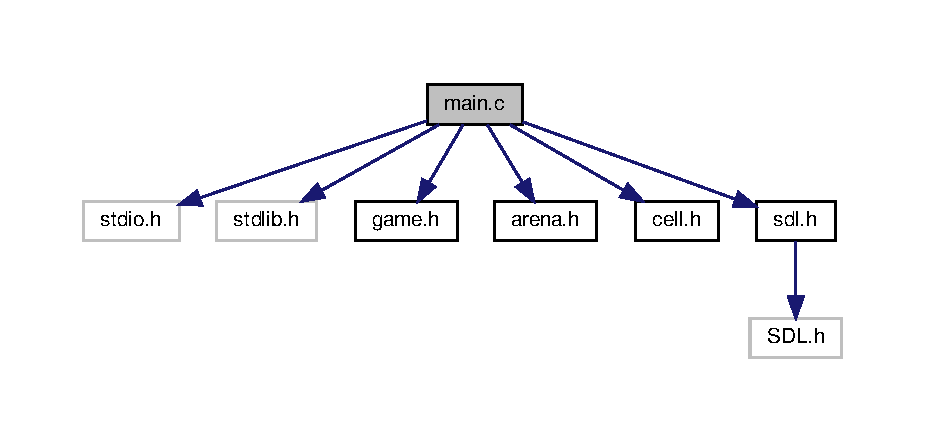
\includegraphics[width=350pt]{main_8c__incl}
\end{center}
\end{figure}
\subsection*{Functions}
\begin{DoxyCompactItemize}
\item 
int \hyperlink{main_8c_a0ddf1224851353fc92bfbff6f499fa97}{main} (int argc, char $\ast$argv\mbox{[}$\,$\mbox{]})
\end{DoxyCompactItemize}


\subsection{Function Documentation}
\mbox{\Hypertarget{main_8c_a0ddf1224851353fc92bfbff6f499fa97}\label{main_8c_a0ddf1224851353fc92bfbff6f499fa97}} 
\index{main.\+c@{main.\+c}!main@{main}}
\index{main@{main}!main.\+c@{main.\+c}}
\subsubsection{\texorpdfstring{main()}{main()}}
{\footnotesize\ttfamily int main (\begin{DoxyParamCaption}\item[{int}]{argc,  }\item[{char $\ast$}]{argv\mbox{[}$\,$\mbox{]} }\end{DoxyParamCaption})}


%--- End generated contents ---

% Index
\backmatter
\newpage
\phantomsection
\clearemptydoublepage
\addcontentsline{toc}{chapter}{Index}
\printindex

\end{document}
